\documentclass[12pt]{article}
\usepackage[utf8]{inputenc}
\usepackage{amsmath, amssymb, amsthm}
\usepackage{graphicx}
\usepackage{booktabs}
\usepackage{geometry}
\usepackage{hyperref}
\usepackage{caption}

\usepackage{listings}
\usepackage{xcolor} % Required for color highlighting

% 1. Define your syntax colors
\definecolor{commentcolor}{rgb}{0, 0.6, 0}       % Green comments
\definecolor{keywordcolor}{rgb}{0, 0, 1}         % Blue keywords
\definecolor{stringcolor}{rgb}{0.63, 0.13, 0.94} % Purple strings
\definecolor{numbercolor}{rgb}{0.5, 0.5, 0.5}     % Gray line numbers

% 2. Configure the monospace and color settings
\lstset{
    basicstyle=\ttfamily\small,        % Forces a clean, pure monospace font
    commentstyle=\color{commentcolor}\itshape , % Applies color to comments
    keywordstyle=\color{keywordcolor}\bfseries, % Colored & bold keywords
    stringstyle=\color{stringcolor},   % Applies color to strings
    %
    numbers=left,                      % Puts line numbers on the left
    numberstyle=\tiny\color{numbercolor}, % Tiny gray line numbers
    stepnumber=1,                      % Number every line
    showstringspaces=false,            % Removes awkward underscores in strings
    tabsize=4,                         % Sets default tab width to 4 spaces
    breaklines=true                    % Automatically wraps long lines
}

\geometry{margin=1in}

\usepackage{fancyhdr}
\pagestyle{fancy}
\fancyhf{}

\fancyfoot[L]{\small \textit{Data/Models, Bryan}}
\fancyfoot[C]{\thepage}
\fancyfoot[R]{\small \textit{Last Edit: 7/17/2026}}

\renewcommand{\headrulewidth}{0pt}
\renewcommand{\footrulewidth}{0pt}

\title{Fitting Data to Models}
\author{Sean Bryan\\\textit{Arizona State University}}
\date{}

\begin{document}

\maketitle

\thispagestyle{fancy}

\section{The Average as a ``Best Fit Model''}

Before getting into the weeds with math, it is worthwhile to step back and motivate a fairly common sense result. Why is taking the average of a group of numbers a good idea?

Concretely, let's say we measured the height in inches of each of a group of people, and put them into an array called $x$:
\begin{equation}
x = [67,61,64,62,60].
\end{equation}
Here the entire collection of heights is $x$, and the $i$-th item in the array is $x_i$. So in this case (starting counting from zero like the python programming language does) $x_2$ is 64.

The simplest possible model for this data would be to assert that there really is a single ``true'' height $h$ and that the variations from person to person we see are just random. We need to determine what number we should put in for $h$ in our model.

Whatever $h$ we choose should have the smallest possible difference from the data. To make the math work out better later in the process, let us calculate the total difference between the model and our data by calculating the sum of the squares of the differences. (In math, physics and statistics this quantity mysteriously gets called $\chi^2$, that is ``chi squared,'' and in machine learning and AI it gets called the ``cost function,'' so to make the later equations cleaner let's call this quantity $C$.) This is:
\begin{equation}\label{eq:fancyCmean}
C(h) = \sum_{i=0}^{N-1} (x_i - h)^2
\end{equation}
where $N$ is the number of elements in the array $x$. Writing this out verbosely for the case of our array of five heights, this is:
\begin{equation}
C(h) = (67-h)^2 + (61-h)^2 + (64-h)^2 + (62-h)^2 + (60-h)^2.
\end{equation}
A plot of this function for our particular case is shown in Figure~\ref{fig:chi2}

\begin{figure}
    \centering
    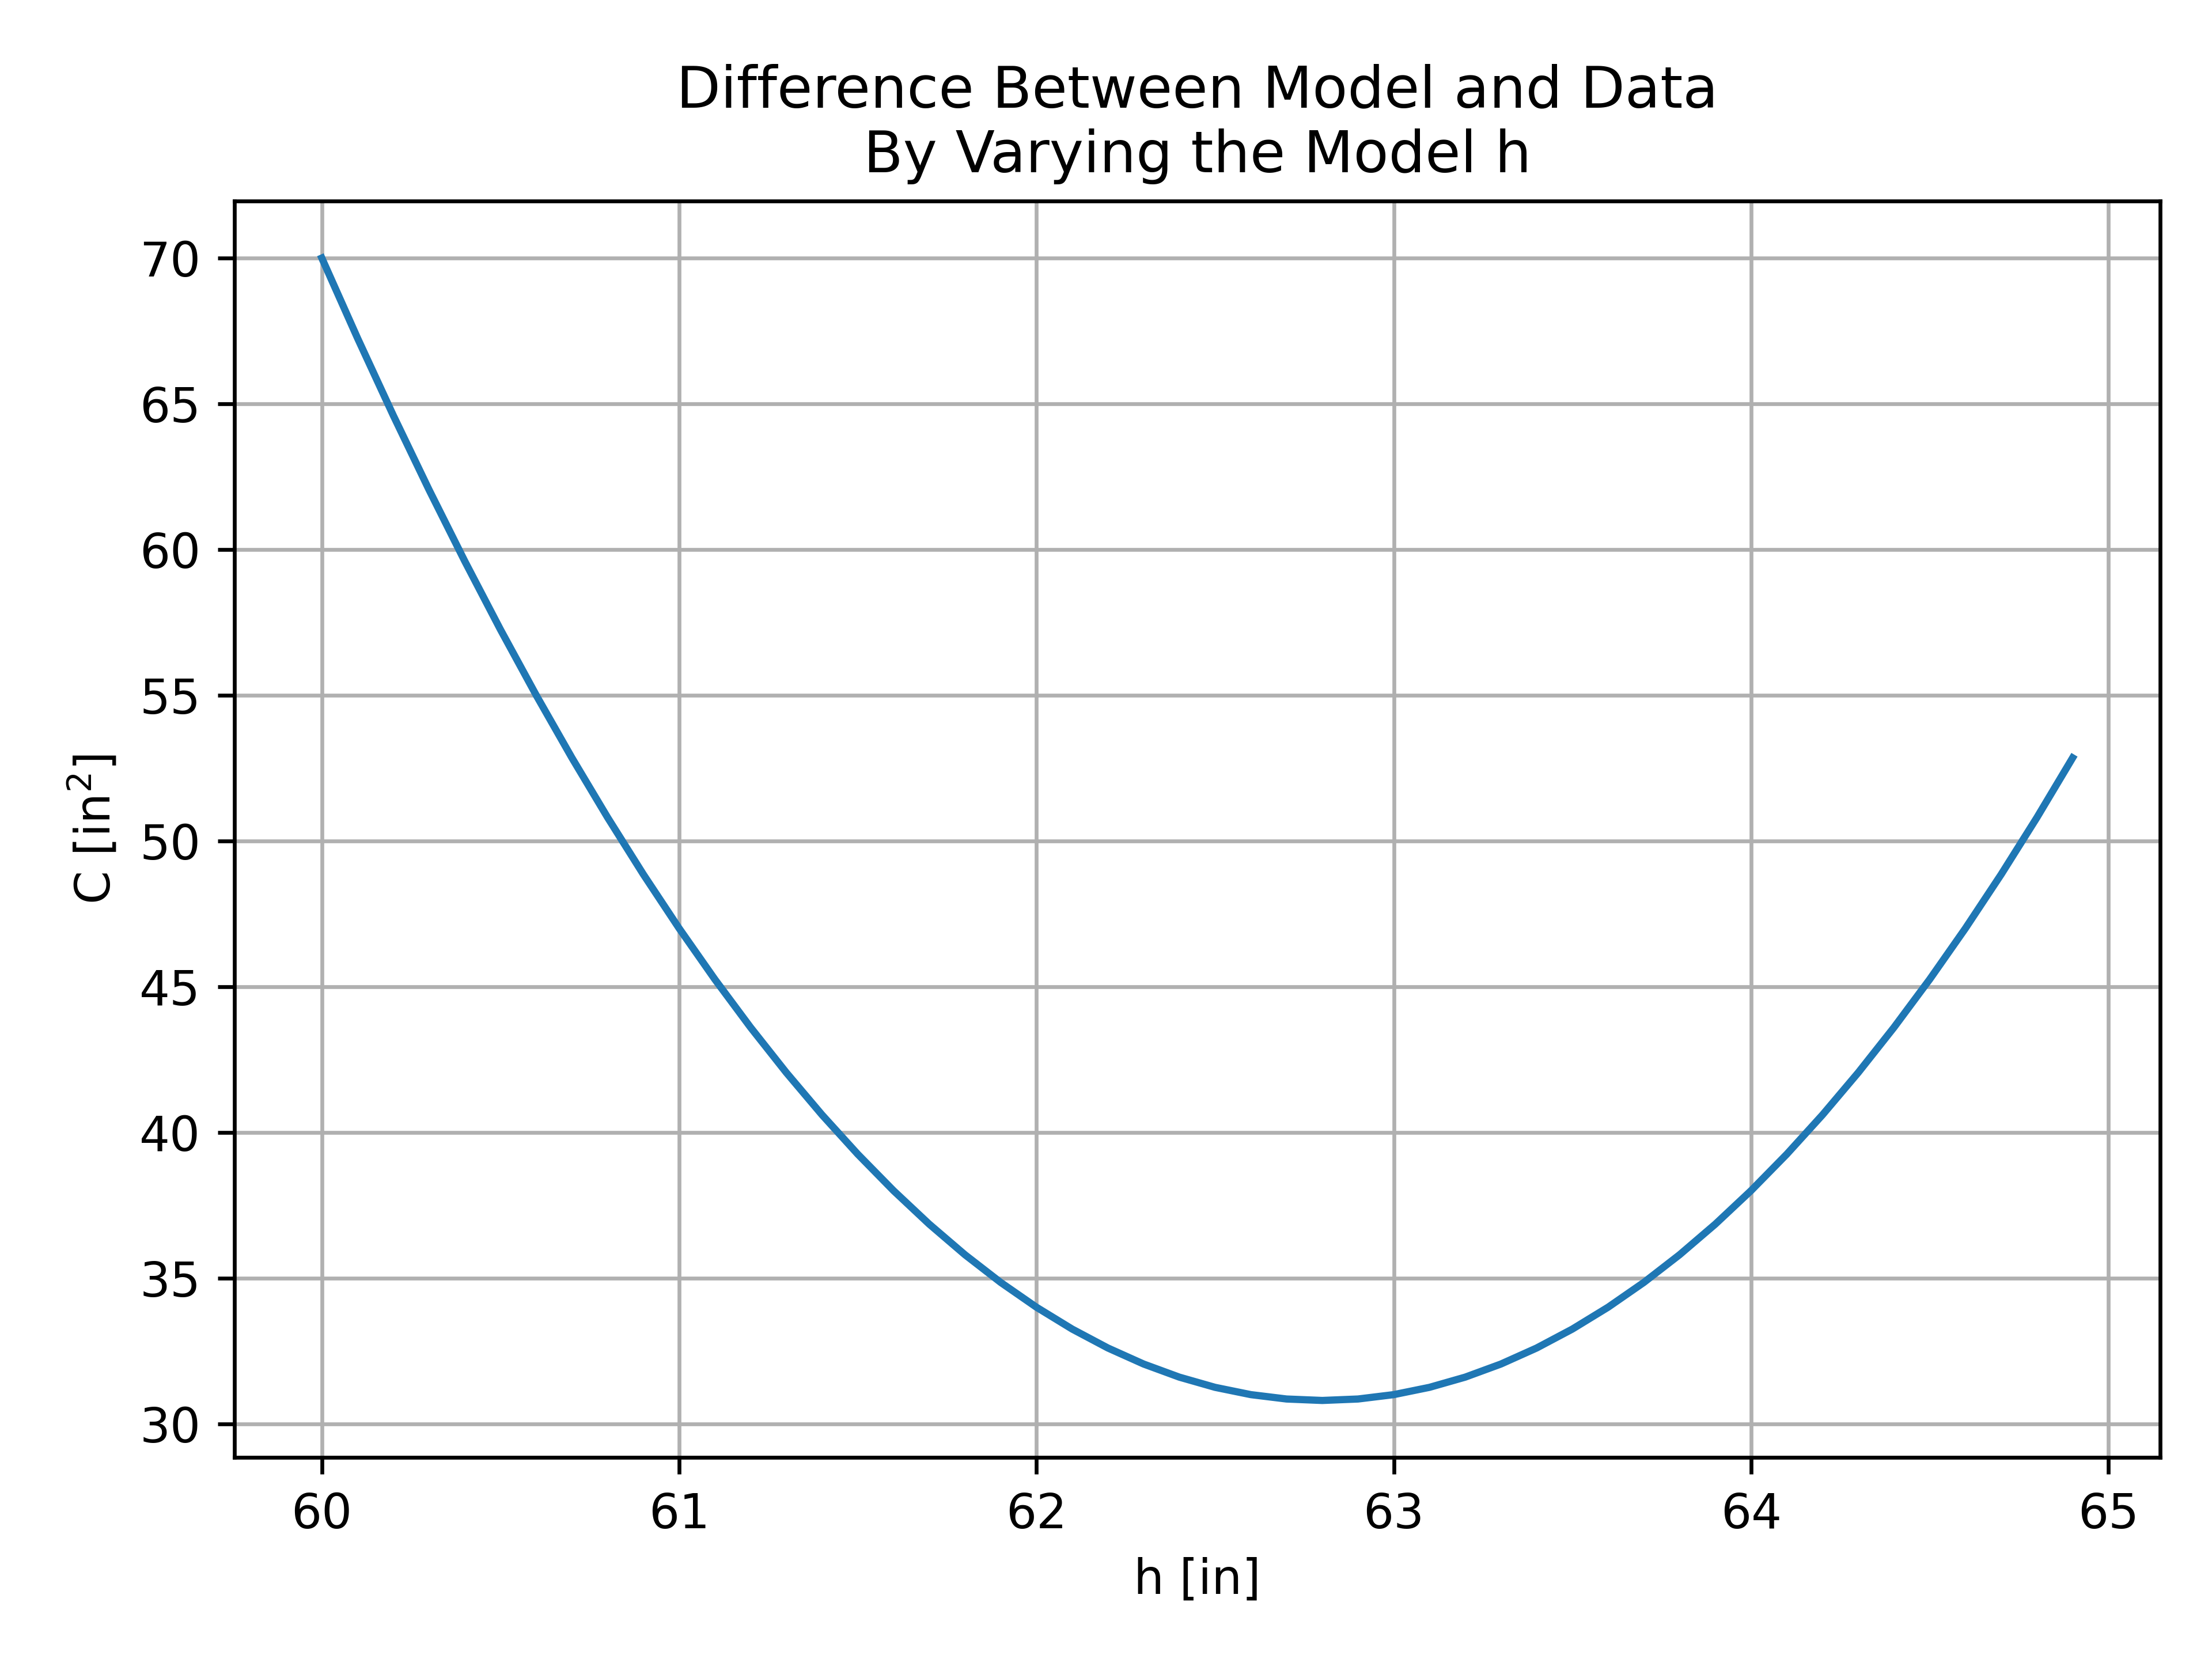
\includegraphics[width=0.5\textwidth]{f1.png}
    \caption{Plot of the sum of the squares of (model-data) for the case of the height data.}
    \label{fig:chi2}
\end{figure}

The best value for $h$ would be the one that has the smallest error $C(h)$. By eye in Figure~\ref{fig:chi2} this looks like it is a little below 63. Note that the derivative of this function $C$ with respect to the model parameter $h$ is zero at this minimum. So, if we want a formula for this minimum, we should calculate $dC/dh$, set it equal to zero, and solve for $h$.

Taking the derivative of the verbose version, and setting it equal to zero, yields:
\begin{equation}
\frac{dC}{dh} = -2(67-h) - 2(61-h) - 2(64-h) - 2(62-h) - 2(60-h) = 0.
\end{equation}
Diividing both sides by $-2$ for clarity, collecting all of the $h$ values on one side, and the number values on the other, yields:
\begin{equation}
(67+61+64+62+60) = 5h
\end{equation}
That leaves $h = (67+61+64+62+60)/5 =62.8$ inches.

In the abstract, let's return to the original problem where we had in general $N$ numbers in the array $x$. Taking the derivative of the fancy formula for $C$ back in Equation~\ref{eq:fancyCmean} yields:
\begin{equation}
\frac{dC}{dh} = -2 \sum_{i=0}^{N-1} (x_i - h) = 0.
\end{equation}
Dividing by -2 again, and moving the $x_i$ terms to one side, and the $h$ terms to the other, yields
\begin{equation}
\sum_{i=0}^{N-1} x_i = \sum_{i=0}^{N-1} h.
\end{equation}
Adding up the constant values on the right yields $N\times h$, so solving for $h$ yields
\begin{equation}
h = \frac{\sum_{i=0}^{N-1} x_i}{N}.
\end{equation}
This formula is just the formula for taking the mean of an array, that is it asks us to add up all the values in $x$ and divide by $N$. But this derivation shows that the mean is the value that has the smallest difference to all of the individual elements in a data set. It is the ``best-fit'' model of a dataset that you model as being truly a single number, plus some random fluctuations.

\section{Linear Fitting}

The math is a little messier, but this same approach can be used to adjust model parameters to minimize the difference $C$ between a model and data even for models that have many parameters. (Indeed, this is how generative AI models are trained, their billions of parameters are adjusted to minimize the difference between the text the model puts out and the training data the creator of the model has access to.)

Following the treatment in Garcia's ``Numerical Methods for Physics'' and in Bevington and Robinson's ``Data Reduction and Error Analysis for the Physical Sciences,'' let's derive and use the formula for a linear fit. The data now has both $x$ and $y$ arrays, each with $N$ datapoints, as plotted in Figure~\ref{fig:fit}. As a concrete example, consider that each $x$ value is the number of items on a plate at a restaurant, and each $y$ value is the price of that plate (in dollars).
\begin{equation}
\begin{array}{r @{\;} c @{\;} l @{\;} r @{\quad} r @{\quad} r @{\quad} r @{\quad} r @{\;\,} l}
x & = & [ & 1, & 2, & 4, & 5, & 7 & ] \\
y & = & [ & 3.49, & 4.62, & 8.53, & 10.51, & 15.32 & ]
\end{array}
\end{equation}

We now assert that our model $y^{model}$ for the price is that there is a constant fixed price for serving the plate to the table, plus a per-item cost for each item on the plate. That, is our model is $y^{model} = mx + b$ where $b$ is the fixed price for serving the plate, and $m$ is the per-item cost. We have to select values for $m$ and $b$ in our model.

Just as before, we write out the sum of the squared of the difference between our model and the data. For this case, that is
\begin{equation}
C(m,b) = \sum_{i=0}^{N-1} (y_i - y^{model}_i)^2 = \sum_{i=0}^{N-1} \left(y_i - (mx_i + b) \right)^2
\end{equation}
It is harder to visualize, but we will vary both $m$ and $b$ to find the combination of both that yields the lowest $C(m,b)$, and this combination of $m$ and $b$ will be the best-fit. At this two-dimensional minimum, the derivative of $C(m,b)$ with respect to $m$, and also with respect to $b$, both will be zero. Calculating that out yields
\begin{eqnarray}
\frac{dC}{dm} &=& -2 \sum_{i=0}^{N-1} \left(y_i - (mx_i + b) \right) x_i = 0 \\ \nonumber
\frac{dC}{db} &=& -2 \sum_{i=0}^{N-1} \left(y_i - (mx_i + b) \right) = 0.
\end{eqnarray}
This looks messy, but as before let's divide everything by $-2$ for clarity, and collect some terms.
\begin{eqnarray}
\sum_{i=0}^{N-1} y_i x_i - m \sum_{i=0}^{N-1} x_i x_i - b \sum_{i=0}^{N-1} x_i &=& 0 \\ \nonumber
\sum_{i=0}^{N-1} y_i - m \sum_{i=0}^{N-1} x_i - \sum_{i=0}^{N-1} b &=& 0.
\end{eqnarray}
It still looks messy, but we can compute some of the sums over the data values $x$ and $y$ ``offline'' and give them names. Let's define several variables, and add the actual numerical value for each for this particular dataset. Define $Sx \equiv \sum x_i = 19$, $Sy \equiv \sum y_i = 42.47$, $Sxy \equiv \sum x_i y_i = 206.64$, and $Sxx \equiv \sum x_i x_i = 95$. Again, these are each just a single number, not an array or function or anything else complicated like that. This lets us rewrite the equations as
\begin{eqnarray}
Sxy &=& m \times Sxx + b\times Sx \\ \nonumber
Sy  &=& m \times Sx + b \times N.
\end{eqnarray}
This is a ``two equations, two unknowns'' situation, so leaving the details of the solution aside, yields
\begin{eqnarray}
m &=& \frac{N\times Sxy - Sy \times Sx}{N \times Sxx - (Sx)^2} \\ \nonumber
b &=& \frac{Sy\times Sxx - Sx \times Sxy}{N \times Sxx - (Sx)^2}.
\end{eqnarray}
Plugging in the specific numbers for our case yields the actual best-fit slope and offset values for our specific case
\begin{eqnarray}
m &=& \frac{5\times 206.64 - 42.47 \times 19}{5 \times 95 - (19)^2} \approx 1.985 \\ \nonumber
b &=& \frac{42.47\times 95 - 19 \times 206.64}{5 \times 95 - (19)^2} \approx 0.952.
\end{eqnarray}
Plotting this line over the data on Figure~\ref{fig:fit} shows that indeed the line does go through the data well.

\begin{figure}
    \centering
    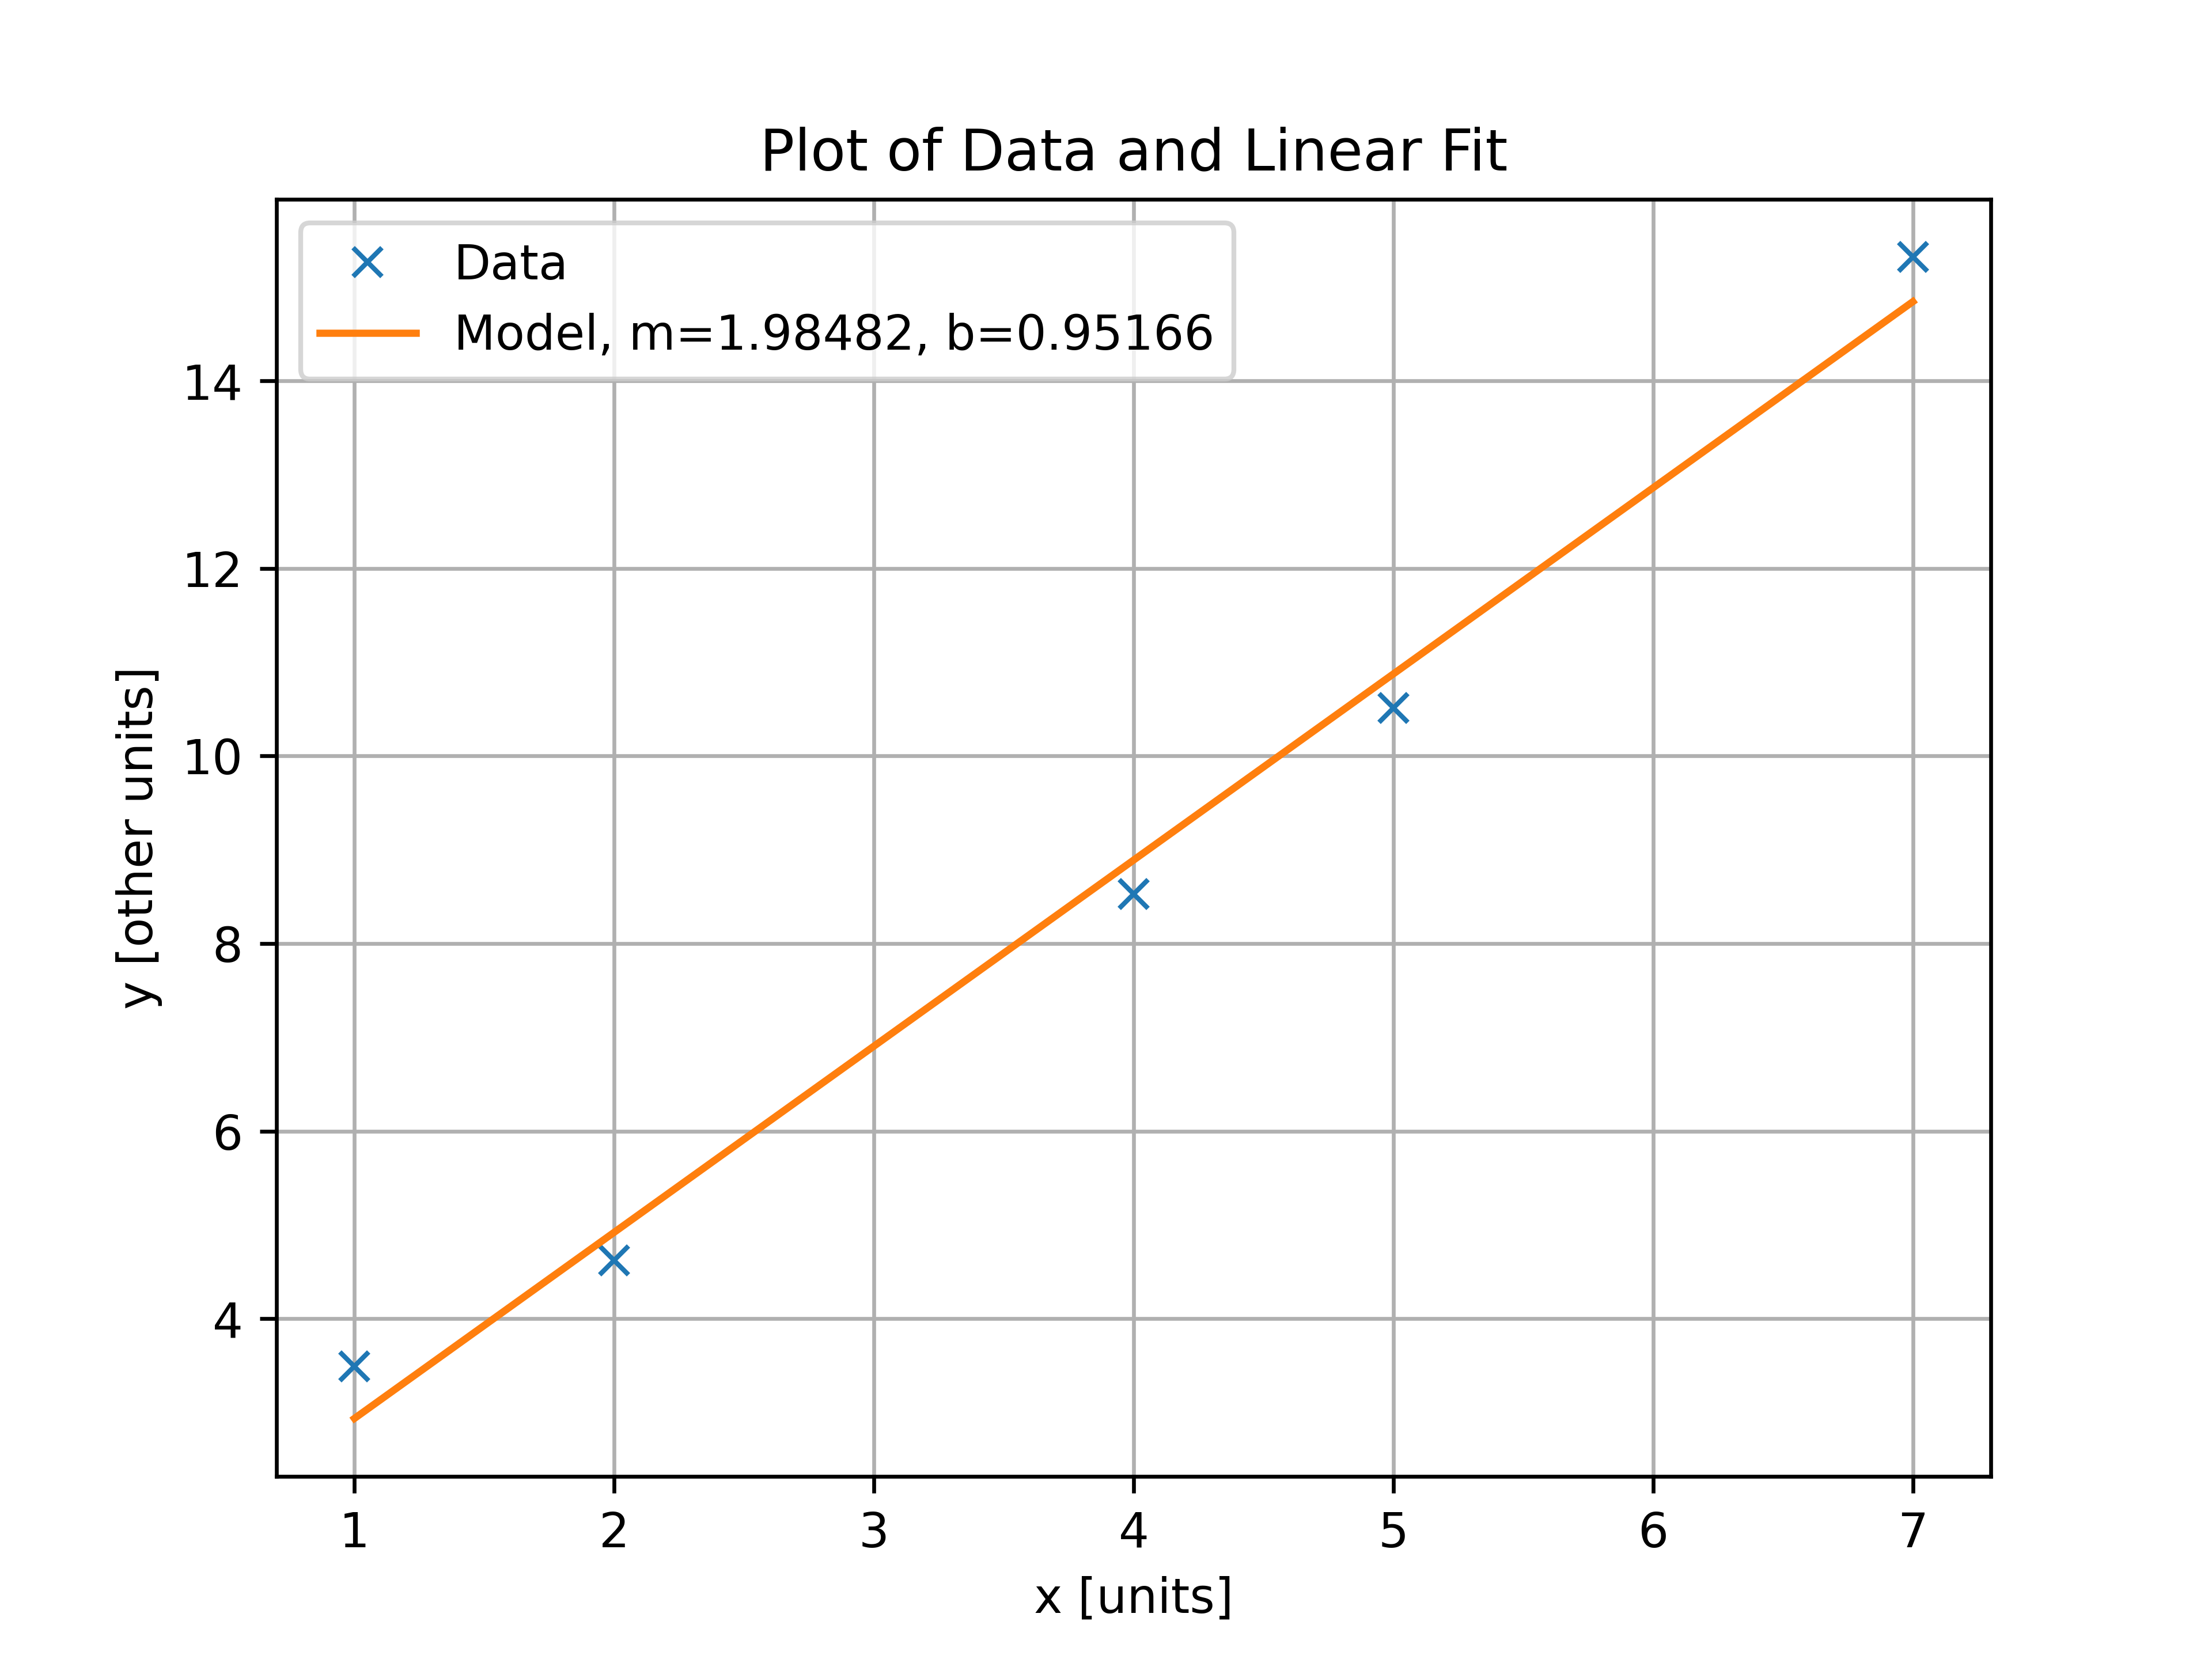
\includegraphics[width=0.5\textwidth]{f2.png}
    \caption{Plot of data and a linear fit.}
    \label{fig:fit}
\end{figure}

Stepping back, this is a minor miracle! After some calculus, we were able to add together different combinations of the numbers in our data to get the best fit line. No AI needed! As you can read in the literature in the ``Further Work'' section, this approach can be further generalized to any function that is a linear combination of templates. That includes polynomials, waves of different frequencies, templates of measured data, or a wide range of other situations.

\section{Computer Program}

Again, this can all be calculated by hand or with a calculator, there is no magic here. You can also plot the data and the model by hand on graph paper. However, it is very convenient with larger datasets to have a computer program to calculate these formulas automatically, and plot the data automatically.

At the end of this document is a listing for a python program that does all of this. Read it, see how it implements the equations, type it in, and try running it to reproduce Figure~\ref{fig:fit}. Try putting your own different data in for $x$ and $y$ and see what you get.

\section{Further Work}

Garcia's book ``Numerical Methods for Physics'' has an excellent section about fitting models to data. The documentation for \texttt{scipy} also has great information. In addition, \texttt{scikit-learn} has a powerful and usable collection of machine learning/neural network tools. On your own, look into general linear fitting (Garcia's book has a great derivation), non-linear fitting (the function \texttt{curve\_fit} in \texttt{scipy} is a great tool for this and has good documentation, or \texttt{emcee} has a much fancier approach), and neural networks (start by going to \texttt{playground.tensorflow.org} and interacting with it, then later read up on \texttt{scikit-learn} neural network regression and classification and try examples).

\newpage
\begin{lstlisting}[language=Python, caption={Listing of a python program to do a linear fit. Note that the line numbers in grey at the left are for reference, and should not be typed in to the program.}]
import numpy as np
import matplotlib.pyplot as pl

# create the data arrays x and y
x = np.array([1,2,4,5,7])
y = np.array([3.49,4.62,8.53,10.51,15.32])

# calculate the sum quantities
N = len(x)
Sx = np.sum(x)
Sy = np.sum(y)
Sxx = np.sum(x*x)
Sxy = np.sum(x*y)

# calculate the best-fit slope and offsets
m = (N*Sxy  - Sy*Sx)  / (N*Sxx - Sx**2)
b = (Sy*Sxx - Sx*Sxy) / (N*Sxx - Sx**2)

# make a plot of the data and the fit
# create the figure
pl.figure()
# plot the actual two traces
pl.plot(x,y,'x',label='Data')
pl.plot(x,m*x + b,'-',label='Model, m='+str(m)+', b='+str(b))
# add labels to the axes
pl.xlabel('x [units]')
pl.ylabel('y [other units]')
# add a title
pl.title('Plot of Data and Linear Fit')
# show the legend
pl.legend()
# add a grid
pl.grid('on')
# show it to the screen
pl.ion()
pl.show()
\end{lstlisting}

\end{document}
